\documentclass{article}
\usepackage{amsmath} %This allows me to use the align functionality.
                     %If you find yourself trying to replicate
                     %something you found online, ensure you're
                     %loading the necessary packages!
\usepackage{amsfonts}%Math font
\usepackage{graphicx}%For including graphics
\usepackage{hyperref}%For Hyperlinks
\usepackage[shortlabels]{enumitem}% For enumerated lists with labels specified
                                  % We had to run tlmgr_install("enumitem") in R
\hypersetup{colorlinks = true,citecolor=black} %set citations to have black (not green) color
\usepackage{natbib}        %For the bibliography
\setlength{\bibsep}{0pt plus 0.3ex}
\bibliographystyle{apalike}%For the bibliography
\usepackage[margin=0.50in]{geometry}
\usepackage{float}
\usepackage{multicol}

%fix for figures
\usepackage{caption}
\newenvironment{Figure}
  {\par\medskip\noindent\minipage{\linewidth}}
  {\endminipage\par\medskip}
\begin{document}

\vspace{-1in}
\title{Lab 1 -- MATH 240 -- Computational Statistics}

\author{
  First Author \\
  Affiliation  \\
  Department  \\
  {\tt email@domain}
}

\date{}

\maketitle

\begin{multicols}{2}
\begin{abstract}
This document provides a basic template for the 2-page labs we will complete each week. Here, you should provide a succinct summary about what you did and why it might be helpful.
\end{abstract}

\textbf{Keywords:} What topics does the lab cover with respect to class?

\section{Instructions}
\noindent For this lab, you will 
\begin{enumerate}[1.]\itemsep0em
\item Install \href{https://cran.rstudio.com/}{R} and \href{https://cran.rstudio.com/}{RStudio}
\item Install tinytex (if necessary): \\\texttt{install.packages("tinytex")}
\item Create a GitHub account \href{https://github.com/}{here}, and email me your user-name.
\item Install \href{https://desktop.github.com/}{GitHub desktop}
\item Accept the LAB 1 assignment \href{https://classroom.github.com/a/gfC_xMMl}{here}.
\item Recreate this document (except put your name/info at the top) to get used to writing in LATEX~ and to see the types of things we can do when creating a document to convey statistical information. Make sure to commit and push your work using GitHub desktop as you finish each section.
\end{enumerate}
\noindent \textbf{Remark:} You will find the class Sweave cheatsheet to be \emph{incredibly} \verb|(\emph{incredibly})| helpful.
\section{Word Processing Tasks}
\subsection{Centering Text}
\begin{center}
We can center text in Sweave.
\end{center}
\subsection{Bold, Italics, and Underlining}
\noindent We can \textbf{bold}, \textit{italicize}, \underline{underline}, and \emph{emphasize} text in Sweave. \\Note, I did a column break here so that the list wasn't broken across columns. 
\columnbreak
\subsection{Lists, and Numbered Lists}
\noindent We can write an unordered list in Sweave.
\begin{itemize}\itemsep0em
\item first item
\item second item
\item third item
\end{itemize}
We can write a numbered list in Sweave
\begin{enumerate}[1.]\itemsep0em
\item first item
\item second item
\item third item
\end{enumerate}
We can write a lettered list in Sweave
\begin{enumerate}[a.]\itemsep0em
\item first item
\item second item
\item third item
\end{enumerate}
\subsection{Submissions}
\noindent This part of the mideterm is due Sunday November 14 by 5p. I will not accept late submissions. Note that you may use this template to help build your introduction and methods sections, and you can use the work you did as a group during the datathon. Still, I expect this submission to be your own summary and extension of that work without collaboration.
\subsection{Typing Mathematical Equations}
\noindent We can write a one line equation that is centered like this
\[\widehat{y_i} = \beta_0 + \beta_1 x_{1i}+ \beta_2 x_{2i} + \beta_3 x_1i x_2i + \epsilon_i.\]\\
\noindent This can be written in the text, as $\widehat{y_i} = \beta_0 + \beta_1 x_{1i}+ \beta_2 x_{2i} + \beta_3 x_1i x_2i + \epsilon_i$ using as well.\\
When we need to show multiple steps, we can create a multi-line equation that is centered like this:
\begin{align*}
8(x-5)+x&=9(x-5)+5\\
8x-40+x&=9x-45+15 \tag{Distributing}\\
9x-40&=9x-40 \tag{Combining like terms}\\
9x&=9x \tag{Adding 40 to both sides}\\
x=x \tag{Dividing both sides by 9}\\
\end{align*}
\begin{quote}
\noindent The equality holds for any x.\\
Note, I did a page break here so that the next section started on a clean page.
\newpage
\subsection{Running R Code}
\noindent Code chunks can be entered into Sweave; e.g., here are some comments.
\scriptsize
\begin{knitrout}
\definecolor{shadecolor}{rgb}{0.969, 0.969, 0.969}\color{fgcolor}\begin{kframe}
\begin{alltt}
\hlcom{# R code goes here}
\hlcom{# Output is automatically printed in the pdf}
\end{alltt}
\end{kframe}
\end{knitrout}
\normalsize
Below, you see that we can do algebra with R.
\scriptsize
\begin{knitrout}
\definecolor{shadecolor}{rgb}{0.969, 0.969, 0.969}\color{fgcolor}\begin{kframe}
\begin{alltt}
\hlnum{8}\hlopt{*}\hldef{(}\hlnum{9}\hlopt{-}\hlnum{5}\hldef{)} \hlopt{+} \hlnum{9} \hlcom{# 8(x-5) + x for x=9}
\end{alltt}
\begin{verbatim}
## [1] 41
\end{verbatim}
\end{kframe}
\end{knitrout}
\normalsize
Alternatively, we can produced the output without the code.
\scriptsize
\begin{knitrout}
\definecolor{shadecolor}{rgb}{0.969, 0.969, 0.969}\color{fgcolor}\begin{kframe}
\begin{verbatim}
## [1] 41
\end{verbatim}
\end{kframe}
\end{knitrout}
\normalsize
Below, we show we can produced the code without evaluating it.
\scriptsize
\begin{knitrout}
\definecolor{shadecolor}{rgb}{0.969, 0.969, 0.969}\color{fgcolor}\begin{kframe}
\begin{alltt}
\hlnum{8}\hlopt{*}\hldef{(}\hlnum{9}\hlopt{-}\hlnum{5}\hldef{)} \hlopt{+} \hlnum{9}
\end{alltt}
\end{kframe}
\end{knitrout}
\normalsize
We can also call objects from R directly.
\scriptsize
\begin{knitrout}
\definecolor{shadecolor}{rgb}{0.969, 0.969, 0.969}\color{fgcolor}\begin{kframe}
\begin{alltt}
\hldef{result} \hlkwb{<-} \hlnum{8}\hlopt{*}\hldef{(}\hlnum{9}\hlopt{-}\hlnum{5}\hldef{)} \hlopt{+} \hlnum{9} \hlcom{# 8(x-5) + x for x = 9}
\hldef{result.with.error} \hlkwb{<-} \hldef{result} \hlopt{+} \hlkwd{rnorm}\hldef{(}\hlnum{1}\hldef{,} \hlkwc{mean} \hldef{=} \hlnum{0}\hldef{,} \hlkwc{sd} \hldef{=} \hlnum{0.1}\hldef{)}
\hldef{result.with.error}
\end{alltt}
\begin{verbatim}
## [1] 40.99104
\end{verbatim}
\end{kframe}
\end{knitrout}
\normalsize
The result is 40.9910426. Note that I did not type the result, but I used the command.
\subsection{Plotting}
\noindent We can also plot with R.
\scriptsize
\begin{knitrout}
\definecolor{shadecolor}{rgb}{0.969, 0.969, 0.969}\color{fgcolor}\begin{kframe}
\begin{alltt}
\hlcom{#Plot a histogram of random exponential data}
\hlkwd{hist}\hldef{(}\hlkwd{rexp}\hldef{(}\hlnum{100}\hldef{))}
\end{alltt}
\end{kframe}
\end{knitrout}
\normalsize
\begin{figure}[H]
\begin{center}
%This code is evaluated, but not printed
%warning=FALSE and message=FALSE ensure no text is returned as a by product of
%printing; this would cause an error in that plot+text is returned instead of
%just the plot
\begin{knitrout}
\definecolor{shadecolor}{rgb}{0.969, 0.969, 0.969}\color{fgcolor}
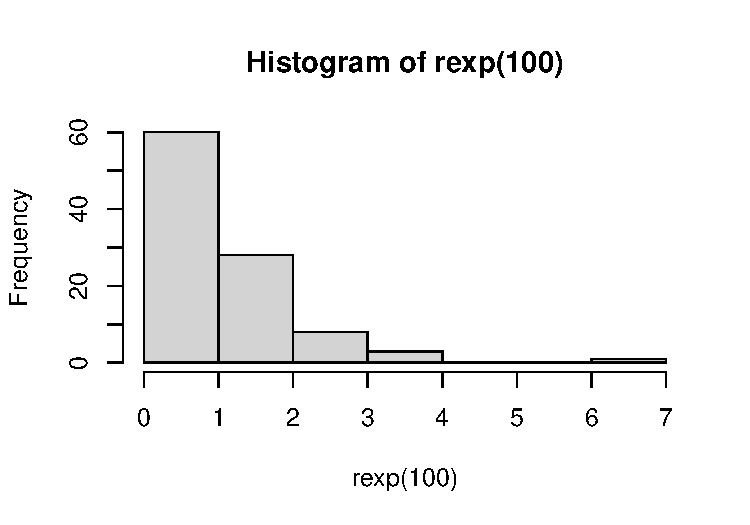
\includegraphics[width=\maxwidth]{figure/unnamed-chunk-6-1} 
\end{knitrout}
\caption{A histogram of random exponentially distributed data, $n=100$.}
\label{plot1} %we can now reference plot1
\end{center}
\end{figure}
\columnbreak
\subsection{Tables}
\noindent
Below, we load and take a peek at some data about the death rates per 1000 in Virginia in 1940 (Molyneaux et al., 1947).
\scriptsize
\begin{knitrout}
\definecolor{shadecolor}{rgb}{0.969, 0.969, 0.969}\color{fgcolor}\begin{kframe}
\begin{alltt}
\hlkwd{data}\hldef{(VADeaths)}
\hlkwd{head}\hldef{(VADeaths)} \hlcom{# Take a peek of the data}
\end{alltt}
\begin{verbatim}
##       Rural Male Rural Female Urban Male Urban Female
## 50-54       11.7          8.7       15.4          8.4
## 55-59       18.1         11.7       24.3         13.6
## 60-64       26.9         20.3       37.0         19.3
## 65-69       41.0         30.9       54.6         35.1
## 70-74       66.0         54.3       71.1         50.0
\end{verbatim}
\end{kframe}
\end{knitrout}





